

Voici un tableau de variations.

\begin{tikzpicture}
\tkzTabInit[lgt=1,espcl=2]{ $x$ / 1,$f $ / 2}
{ $-\infty$ , $1$ ,$+\infty$}
\tkzTabVar{-/$ $,+/$10$,-/$ $ }
\end{tikzpicture}


Parmi les expressions suivantes, qui est $f$ ?
\begin{tabular}{cc}
A. $(x-1)^2+10$ & B. $(x+1)^2+10$\\
C. $-(x-1)^2+10$ & D. $x^2-2x+11$ \\ 
\end{tabular} 